%\documentclass[12pt,handout]{beamer}
\documentclass[xcolor=dvipsnames,presentation]{beamer}
\usepackage{../oop-slides-lab}

\setbeamertemplate{bibliography item}[text]

\newcommand{\lab}{Lab04}

\title[{\lab} -- DVCS1]{Introduzione ai Distributed Version Control Systems
\\ Visualizzazione della storia dello sviluppo con git}

\date[\today]{\today}

\immediate\write18{./download-resources.sh}

\begin{document}

\frame[label=coverpage]{\titlepage}

\section{Decentralized version control systems I}

\subsection{Generalità}

\fr{Cosa sono}{
   I DVCS sono software che consentono di:
   \iz{
      \item Mantenere traccia dei cambiamenti fatti ad un progetto, consentendo di andare ``avanti e
indietro'' nel tempo.
      \item Consentire e promuovere il lavoro di gruppo, anche in parallelo (lo vedremo nel prossimo
lab)
   }

    L'esigenza di poter tornare a salvataggi precedenti è sempre stata avvertita dagli sviluppatori
(e non solo). L'operazione di salvare più stati del proprio lavoro è detta \textit{versioning}, un
software che semplifica il versioning è un \textit{version control system} (o \textit{versioning
system}).
}

\fr{Pillole di storia}{

    Sistemi di versioning:
    \iz {
        \item ``Fai da te'' --- è il sistema che la maggior parte di voi ha usato finora: si fa una
copia di tutti i file in una cartella (magari numerata). Costa molto in spazio ed in tempo, rende
difficile lo scambio di file e il lavoro parallelo.
        \item \emph{CVS} --- Fu il primo sistema di versioning. Studiato per salvare automaticamente
i punti di salvataggio di file di testo. È difficile usarlo per file binari, facilita lo scambio di
file rispetto ad inviarsi cartelle.
        \item \emph{SVN} --- Evoluzione di CVS. Molto più veloce e con supporto nativo a file
binari. Il lavoro in parallelo è possibile a patto di adottare un flusso di lavoro di squadra molto
controllato.
        \item \emph{Git} e \emph{Mercurial} --- Sviluppati parallelamente per superare le
limitazioni di SVN, sono nati praticamente identici. Più veloci di SVN e pensati per supportare il
lavoro massivamente parallelo di team sparsi per il mondo.
    }
}

\fr{Diffusione}{
   Sono usati per tutti i moderni processi di sviluppo software. Un po' di esempi:
   \iz{
      \item Android (git)
      \item Drupal (git)
      \item Facebook (Mercurial)
      \item GCC (git)
      \item Go (git)
      \item Java JDK (Mercurial)
      \item Libreoffice (git)
      \item Linux kernel (git)
      \item Python (git)
      \item VLC Video Player (git)
      \item Wine (git)
      \item le slides e il laboratorio di OOP! (git)
   }
}

\begin{frame}[allowframebreaks]{Diffusione dei sistemi di controllo di versione}
    \begin{center}
        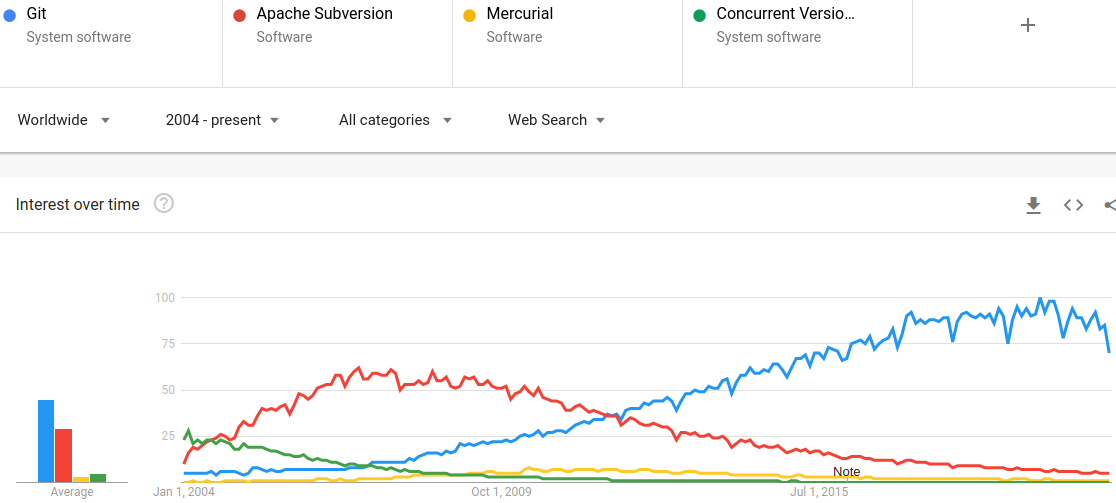
\includegraphics[width=\textwidth, height=.77\textheight, keepaspectratio]{img/gtrends} \\
        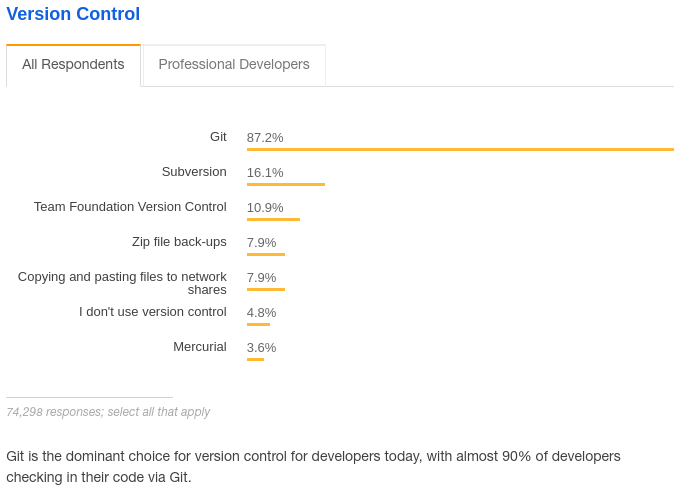
\includegraphics[width=\textwidth, height=.77\textheight, keepaspectratio]{img/stackoverflow} \\
        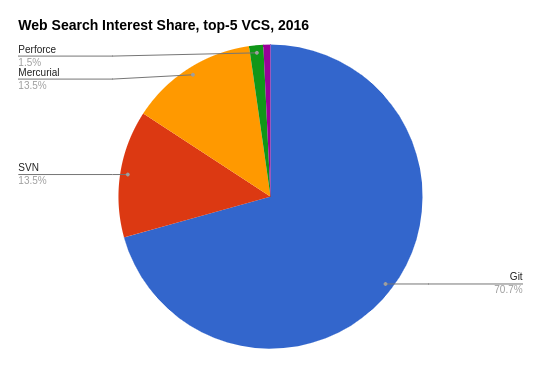
\includegraphics[width=\textwidth, height=.77\textheight, keepaspectratio]{img/interest} \\
        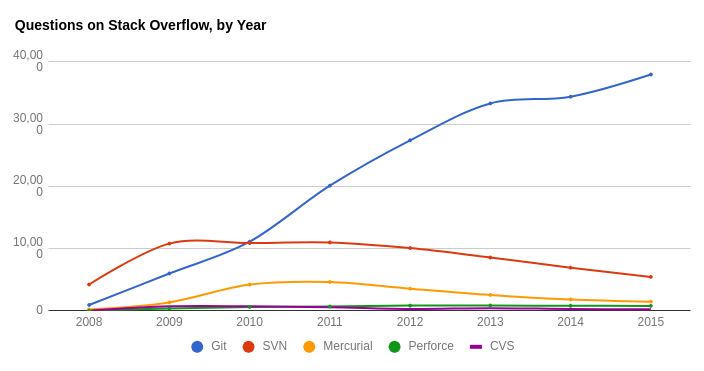
\includegraphics[width=\textwidth, height=.77\textheight, keepaspectratio]{img/questions}\\
        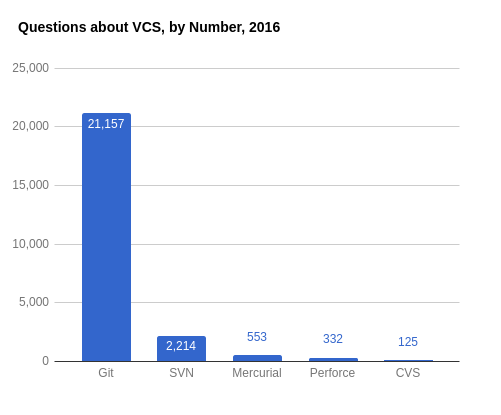
\includegraphics[width=\textwidth, height=.77\textheight,keepaspectratio]{img/questionsbynum} \\
        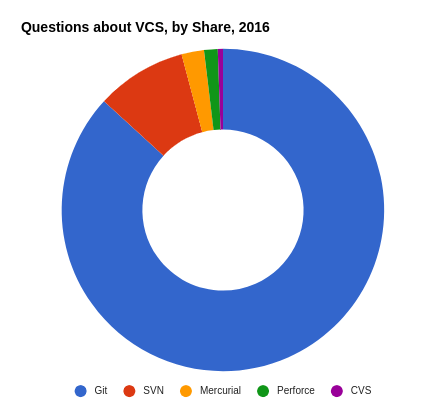
\includegraphics[width=\textwidth, height=.77\textheight,keepaspectratio]{img/questionsbyshare} \\
    \end{center}
\end{frame}

\begin{frame}[fragile]{Bits of history}
    \begin{itemize}
        \item In April 2005, BitKeeper, the SCM Linux was developed with, withdrawn the free (as in
beer) use
        \item No other SCM met the requirements of Torvalds
        \begin{itemize}
            \item Performance was the \textit{real} issue with such a code base
        \end{itemize}
        \item Torvalds decided to write his own
        \item The project was successful, and Torvalds appointed maintenance to Hamano
    \end{itemize}
    \begin{block}{Why the name}
        \begin{quote}
            I'm an egotistical bastard, and I name all my projects after myself. First 'Linux', now
'git'. \footnote{\tiny{From the project Wiki. ``git'' is slang for ``pig headed, think they are
always correct, argumentative''}}
            \begin{flushright}
                \normalfont{--- Linus Torvalds}
            \end{flushright}
        \end{quote}
    \end{block}
\end{frame}

\subsection{Concetti fondamentali}

\begin{frame}[allowframebreaks]{Concetti basilari e terminologia}
    \begin{block}{Repository}
        Il repository è l'insieme dei file che vengono tracciati dal DVCS assieme ai metadati, ossia
alle informazioni che servono a ricostruire qualunque stato precedente.
    \end{block}
    \begin{block}{Tracciamento delle differenze}
Abilità di registrare le differenze fra diverse versioni di uno o più file. Invece di
salvare l'intero stato (tutto il contenuto di un file), vengono salvate solo le informazioni
necessarie a ricostruire il file a partire dal salvataggio precedente.
    \end{block}
    \begin{center}
        \includegraphics[width=\textwidth, height=.77\textheight, keepaspectratio]{img/deltas} \\
    \end{center}
    \framebreak
    \begin{block}{Snapshotting}
Capacità di salvare lo stato di tutti i file che fanno parte del progetto in una sola versione, creando una fotografia del sistema.
    \end{block}
    \begin{center}
        \includegraphics[width=\textwidth, height=.77\textheight, keepaspectratio]{img/snapshots} \\
    \end{center}
\textbf{Nota}: un buon version control system è in grado di esporre sia meccanismi di snapshotting (ad esempio, riporta il repository a tre versioni fa)
e meccanismi basati sulle differenze (ad esempio, dimmi cos'è cambiato in questo file dall'anno scorso).
    \framebreak
    \begin{block}{Commit}
        Salvataggio dello stato del repository
    \end{block}
    \begin{block}{Staging area}
        Insieme delle modifiche accodate per esser salvate al prossimo commit. Il processo di
salvataggio si articola infatti in due fasi:
        \begin{enumerate}
            \item \textbf{Staging} --- Selezione di quali file modificati, aggiunti o rimossi
salvare al prossimo commit
            \item \textbf{Commit} --- Effettivo salvataggio delle modifiche presenti nella staging
area
        \end{enumerate}
    \end{block}
    \begin{block}{Navigazione della storia}
        Possibilità di tornare ad un qualunque commit (salvataggio) precedente o successivo
    \end{block}
\end{frame}

\subsection{Operazioni preliminari}

\begin{frame}[allowframebreaks]{Configurazione globale}
    \bl{In generale}{
        Come ogni prodotto software, i DVCS necessitano di alcune operazioni di configurazione
preliminari. In particolare, richiedono di impostare un nome utente ed una email (in modo da poter
capire chi ha apportato modifiche).
    }
    \bl{In Git}{
        È possibile specificare un nome utente di default utilizzando
        \iz {
            \item \texttt{git config --global user.name "YOUR NAME"}
            \begin{itemize}
                \item \textbf{OVVIAMENTE} al posto di \texttt{YOUR NAME} dovrete inserire il vostro nome.
                \item \textbf{Configurate il vostro vero nome, non un nickname!}
            \end{itemize}
        }
        È possibile specificare una email di default utilizzando
        \iz {
            \item \texttt{git config --global user.email "your.email@provider"}
        }
    }
    \bl{Caratteri di newline}{
        \begin{itemize}
            \item Git prova ad essere ``smart'' nella configurazione dei caratteri che rappresentano
una nuova linea di testo, che differiscono per piattaforma
            \begin{itemize}
                \item Come spesso capita, nel tentativo di essere smart fa più danno che utile.
            \end{itemize}
            \item Noi useremo una precisa configurazione di Eclipse
            \item Vogliamo che i nostri file abbiano un terminatore preciso, e vogliamo che tutti i
membri del team lo usino correttamente
            \begin{itemize}
                \item Evitando di fare mega-salvataggi solo perché cambiano i caratteri di fine
linea
            \end{itemize}
            \item Linux e MacOS: usa il carattere presente nel testo
            \begin{itemize}
                \item \texttt{git config --global core.autocrlf input}
            \end{itemize}
            \item Windows: disattiva la conversione automatica a CRLF
            \begin{itemize}
                \item \texttt{git config --global core.autocrlf false}
            \end{itemize}
        \end{itemize}
    }
    \begin{block}{Esercizio}
        \begin{itemize}
            \item Si apra un terminale
            \item Si settino username ed email di default usando nome e cognome ed email istituzionale
            \item Si disabiliti la funzione autocrlf
        \end{itemize}
    \end{block}
\end{frame}

\section{Gestione di un repository}

\subsection{Operazioni di base sul repository}

\begin{frame}[allowframebreaks]{Inizializzazione di un repository}
    \bl{In generale}{
        È necessario esplicitare che, da un certo punto del file system, si desidera utilizzare il
        DVCS per tener traccia dei cambiamenti dei file contenuti da quel punto del file system.
        \begin{itemize}
            \item Il DVCS dovrà salvare dei metadati che consentano di ricostruire gli stati
            precedenti del sistema
            \item Bisognerà prestare attenzione a quale cartella si inizializza: inizializzare il
            punto sbagliato implicherà repository enormi ed ingestibili!
        \end{itemize}
    }
    \bl{In Git}{
        \iz{
            \item \texttt{git init}
        }
        Marca la cartella corrente come repository Git. Crea una sottocartella nascosta
\texttt{.git} nella quale saranno salvati i metadati.
% Fintanto che la cartella \texttt{.git} è integra, sarà possibile ripristinare lo stato dei file
% del repository a qualunque versione.

        È possibile settare username ed email personalizzati per ogni repository, usando i comandi
visti prima privati dell'argomento \texttt{--global}, e.g.:
        \begin{center}
            \texttt{git config user.email "your.second@email"}
        \end{center}
    }
    \begin{block}{Errori comuni}
        \begin{itemize}
            \item Bisogna posizionarsi dentro la cartella che ospiterà il nostro repository
\textbf{prima} di dare il comando \texttt{git init}
            \item Dare il comando dentro la home folder (dove dovrebbe aprirsi il terminale di
default) marcherà tutta la home folder come repository Git
        \end{itemize}
    \end{block}
    \begin{block}{Esercizio}
        \begin{itemize}
            \item Si crei una cartella di nome \texttt{dvcstest} (comando \texttt{mkdir})
            \item Si entri nella cartella col terminale
            \item Si inizializzi un repository git
            \item Si setti l'email utente \textbf{per il repository} al vostro indirizzo personale
(quindi non quello \texttt{@studio.unibo.it})
            \begin{itemize}
                \item Nota: chi non volesse usare l'indirizzo personale per ragioni di privacy, usi
una email fittizia.
            \end{itemize}
        \end{itemize}
    \end{block}
\end{frame}

\begin{frame}[allowframebreaks,fragile]{Ispezionare lo stato del repository}
    \begin{block}{In generale}
        È necessario sapere quale sia lo stato del repository e della staging area, per conoscere:
        \begin{itemize}
            \item Quali file sono stati modificati
            \item Quali file sono stati aggiunti allo stage
        \end{itemize}
    \end{block}
    \begin{block}{In Git}
        È possibile ispezionare lo stato usando:
        \begin{itemize}
            \item \texttt{git status}
        \end{itemize}
    \end{block}
    \begin{block}{Suggerimenti}
        \begin{itemize}
            \item Bisogna controllare spesso lo stato del repository
            \item Idealmente, prima di ogni operazione che potrebbe modificare lo stato del repository
        \end{itemize}
    \end{block}
    \begin{block}{Esercizio}
        \begin{itemize}
            \item Si ispezioni lo stato corrente del repository
        \end{itemize}
    \end{block}
    \begin{block}{Output atteso}
        \begin{Verbatim}[fontsize=\scriptsize]
On branch master

Initial commit

nothing to commit (create/copy files and use "git add" to track)
        \end{Verbatim}
    \end{block}
    \begin{block}{Spiegazione dell'output}
        \begin{itemize}
            \item Prima linea: il branch su cui ci si trova. Non ne è stato creato nessuno
esplicitamente, quindi Git assume che di default si lavori su un branch di nome \texttt{master}
            \item Seconda linea: Git ci segnala che non abbiamo ancora effettuato alcun commit
            \item Terza linea: Git mostra lo stato della staging area. In questo momento non c'è
nulla di cui far commit (difatti, non ci sono file nel nostro repository)
        \end{itemize}
    \end{block}
\end{frame}

\begin{frame}[allowframebreaks,fragile]{Aggiungere files alla staging area}
    \begin{block}{In generale}
        È necessario segnalare esplicitamente quali file dovranno essere inclusi nel prossimo
salvataggio.
        \begin{itemize}
            \item molti dei file potrebbero essere rigenerabili a partire da altri
            \item Il tracking differenziale è efficiente con file testuali...
            \item ...ma inefficiente con i binari!
            \item tracciare file generabili è uno spreco di risorse!
            \item I file selezionati saranno aggiunti alla ``staging area''
        \end{itemize}
    \end{block}
    \begin{block}{In un progetto Java}
        Vanno tracciati:
        \begin{itemize}
            \item I sorgenti
            \item Le risorse (icone, file di configurazione...)
            \item Librerie copiate nel progetti
            \item Eventuali file esterni, ad esempio un README.md, un file per la licenza, il file .project di Eclipse per facilitare l'import...
        \end{itemize}
        \textbf{Non} vanno tracciati:
        \begin{itemize}
            \item I binari (rigenerabile dai sorgenti)
            \item La documentazione rigenerabile dai sorgenti
            \item Archivi con la vostra applicazione (rigenerabili)
        \end{itemize}
    \end{block}
    \begin{block}{In Git}
        Il sottocomando \texttt{add} aggiunge delle modifiche alla staging area
        \begin{itemize}
            \item \texttt{git add PATH\_TO\_FILE}
            \begin{itemize}
                \item Aggiunge il file indicato alla staging area. Il file deve essere all'interno
del repository.
                \item Il file deve essere cambiato rispetto allo stato precedente (perché nuovo,
modificato, o cancellato)
                \item Il file può essere un file che esisteva ma è stato cancellato!
                \item In questo caso, viene registrata nella staging area la cancellazione
            \end{itemize}
            \item \texttt{git add PATH\_TO\_FILE\_1 PATH\_TO\_FILE\_2 PATH\_TO\_FILE\_N}
            \begin{itemize}
                \item Aggiunge tutti i file indicati alla staging area.
            \end{itemize}
        \end{itemize}
    \end{block}
    \begin{block}{Esercizio}
        \begin{itemize}
            \item All'interno della cartella dove abbiamo inizializzato il repository git vuoto, si
creino due cartelle: \texttt{src} e \texttt{bin}
            \item Si crei dentro src un file \texttt{HelloWorld.java} (ad esempio con Visual Studio Code), contenente un semplice main con una stampa
            \item Si visualizzi lo stato del repository con \texttt{git status}
            \begin{itemize}
                \item Si noti che ci sono nuove informazioni!
                \item Git ci informa che ci sono dei file non tracciati dentro la cartella
\texttt{src/}
            \end{itemize}
            \item Si utilizzi in modo appropriato il comando \texttt{git add} per aggiungere al
tracking il file \texttt{HelloWorld.java}
            \item Se il comando viene eseguito correttamente, non viene dato alcun output all'utente
            \item Si visualizzi lo stato del repository
        \end{itemize}
    \end{block}
    \begin{block}{Output atteso}
        \begin{Verbatim}[fontsize=\scriptsize]
On branch master

Initial commit

Changes to be committed:
  (use "git rm --cached <file>..." to unstage)

        new file:   src/HelloWorld.java
            \end{Verbatim}
    \end{block}
    \begin{block}{Spiegazione dell'output}
        \begin{itemize}
            \item La parte relativa alla staging area è cambiata: git ci segnala che le modifiche ad
\texttt{src/HelloWorld.java} saranno salvate al prossimo commit
        \end{itemize}
    \end{block}
\end{frame}

\begin{frame}[allowframebreaks,fragile]{Creare punti di salvataggio}
    \begin{block}{In generale}
        L'operazione fondamentale che vogliamo eseguire è quella di creare un punto di salvataggio,
che registri i nostri progressi e al quale potremo sempre tornare.

        Assieme al salvataggio, vogliamo registrare alcuni metadati:
        \begin{itemize}
            \item Nome dell'autore del commit
            \item Informazioni per identificare e contattare l'autore (email)
            \item Un \textbf{messaggio} che riassuma quali modifiche sono state fatte in quel commit
            \item Data e ora del commit (acquisite automaticamente)
            \item Un identificativo univoco (hash) (generato automaticamente)
        \end{itemize}

        Il commit non salverà lo stato del progetto, ma il set di modifiche necessarie per portare i
file dallo stato precedente a quello del nuovo commit.
    \end{block}
    \begin{block}{Buone pratiche di commit}
        È molto importante specificare un messaggio di commit sensato.
        \begin{itemize}
            \item Deve essere un breve riassunto di quanto è stato fatto dal salvataggio precedente
            \item Chi vede la storia del progetto deve capire immediatamente quali siano le
differenze che il commit introduce
            \item È buona norma scrivere in inglese usando il simple present
        \end{itemize}
        È molto importante fare commit piccoli e frequenti
        \begin{itemize}
            \item Idealmente, uno ad ogni modifica di cui sia possibile fornire una descrizione
organica nel commit message
            \item Non importa se le modifiche sono minimali
%             \item Ad esempio, i seguenti sono buoni commit:
%             \begin{itemize}
%                 \item \texttt{Aggiunta stampa in caso di errore}, con modifica di una sola linea di
codice
%                 \item \texttt{Aggiunta di final mancanti}, con modifica di poche linee di codice in
un solo file
%                 \item \texttt{Implementata versione iniziale della funzionalità X}, con modifica e
aggiunta di diversi file sorgente
%             \end{itemize}
        \end{itemize}
    \end{block}
    \begin{block}{Cattive pratiche da evitare}
        \begin{itemize}
            \item Messaggi non chiari, generici e/o troppo brevi, ad esempio:
            \begin{itemize}
                \item Fix bug
                \item Fix project
                \item Add files
                \item Commit
            \end{itemize}
            \item Commit giganteschi con molte modifiche, magari non strettamente correlate fra loro
        \end{itemize}
    \end{block}
    \begin{block}{In Git}
        Il sottocomando \texttt{commit} crea il salvataggio
        \begin{itemize}
            \item \texttt{git commit -m "A message"}
            \begin{itemize}
                \footnotesize
                \item Esegue un commit di tutte le modifiche aggiunte alla staging area
                \item Utilizza \texttt{A message} come commit message
            \end{itemize}
            \item \texttt{git commit FILE1 FILE2 FILEN -m "A message"}
            \begin{itemize}
                \footnotesize
                \item Esegue un commit salvando tutte le modifiche ai file elencati
                \item Utilizza \texttt{A message} come commit message
            \end{itemize}
        \end{itemize}
    \end{block}
    \begin{block}{\texttt{commit} senza specificare il messaggio}
        \begin{itemize}
            \item Non è possibile non specificare un messaggio.
            \item Se l'opzione \texttt{-m} viene omessa, viene aperto un editor per l'inserimento
del messaggio
            \item Se il messaggio viene lasciato vuoto, il commit viene rigettato
            \item \texttt{git commit}
            \begin{itemize}
                \footnotesize
                \item Esegue un commit salvando tutte le modifiche nella staging area
                \item Apre l'editor di testo di sistema per l'inserimento del commit message
            \end{itemize}
            \item \texttt{git commit PATH\_TO\_FILE\_1 PATH\_TO\_FILE\_2 PATH\_TO\_FILE\_N}
            \begin{itemize}
                \footnotesize
                \item Esegue un commit salvando tutte le modifiche ai file elencati
                \item Apre l'editor di testo di sistema per l'inserimento del commit message
                \item Equivalente ad eseguire \texttt{git add FILES} seguito da \texttt{git commit}
a partire da una staging area vuota
            \end{itemize}
        \end{itemize}
        Preferite sempre commit con opzione \texttt{-m}, a meno che non abbiate già confidenza con
l'editor di sistema
    \end{block}
    \begin{block}{Configurare l'editor di testo}
        Sistemi diversi hanno editor diversi
        \begin{itemize}
            \item Di default MacOS X utilizza \texttt{vim}
            \item In Linux dipende dalla distribuzione, solitamente è uno fra \texttt{vim},
\texttt{nano}, o \texttt{emacs}
            \item In Windows \textit{dovrebbe} essere \texttt{Notepad.exe} (in laboratorio è
\texttt{vim})
        \end{itemize}
        Non sempre l'editor di default è quello che preferite: è bene configurarlo
        \begin{itemize}
            \item \texttt{git config --global core.editor "editorcommand"}
            \begin{itemize}
                \item Setta \texttt{editorcommand} come comando da invocare per aprire l'editor
                \item Va da sé che il comando debba essere disponibile sul vostro sistema...
            \end{itemize}
        \end{itemize}
        Vi consiglio di:
        \begin{itemize}
            \item Se conoscete già un editor a command line, usate quello
            \item Se non lo avete, in ambiente Linux o Mac, di usare \texttt{nano}
        \end{itemize}
    \end{block}
    \begin{block}{Esercizio}
        \begin{itemize}
            \item Se si sta usando Linux o MacOS X, si configuri adeguatamente l'editor di testo
            \item Si verifichi lo stato del repository
            \item Si effettui il commit delle modifiche presenti nella staging area
            \begin{itemize}
                \item Inserendo un commit message SENSATO!
            \end{itemize}
            \item Si visualizzi lo stato del repository
        \end{itemize}
    \end{block}
    \begin{block}{Output atteso dopo il commit}
        \begin{Verbatim}[fontsize=\scriptsize]
[master (root-commit) 19aa252] Create HelloWorld
 1 file changed, 5 insertions(+)
 create mode 100644 src/HelloWorld.java
\end{Verbatim}
    \end{block}
    \begin{block}{Spiegazione dell'output}
        \begin{itemize}
            \item Ci troviamo nel branch master
            \item Questo è il primo commit (radice)
            \item L'hash del nostro commit (una parte, in realtà) è \texttt{19aa252}
            \begin{itemize}
                \item Ovviamente il vostro potrebbe differire
            \end{itemize}
            \item Il messaggio inserito è ``Create HelloWorld''
            \begin{itemize}
                \item Ovviamente questo è il mio, il vostro potrebbe essere diverso, dipende da che
messaggio avete inserito
            \end{itemize}
            \item È stato modificato un file, in totale sono state inserite 5 righe di codice
            \item È stato creato un nuovo file \texttt{src/HelloWorld.java}
            \begin{itemize}
                \item Si noti che sono stati tracciati i permessi unix (\texttt{644} in ottale)
            \end{itemize}
        \end{itemize}
    \end{block}
\end{frame}

\begin{frame}[allowframebreaks,fragile]{Rimuovere files dalla staging area}
    \begin{block}{In generale}
        Vogliamo poter togliere dalla staging area dei file che abbiamo aggiunto
        \begin{itemize}
            \item Ad esempio perché li abbiamo aggiunti a seguito dell'uso di un comando con la
wildcard
            \item Oppure perché abbiamo deciso di salvare le modifiche in più commit
        \end{itemize}
    \end{block}
    \begin{block}{In Git}
        Il sottocomando \texttt{reset} rimuove delle modifiche \textit{dalla staging area} (non dai
files, a meno di non specificare apposite opzioni)
        \begin{itemize}
            \item \texttt{git reset PATH\_TO\_FILE}
            \begin{itemize}
                \item Rimuove dalla staging area le modifiche fatte al file indicato (non dal
tracking!)
                \item Il file potrebbe anche non esistere, ad esempio se abbiamo cancellato un file
e aggiunto la modifica alla staging area.
            \end{itemize}
            \item \texttt{git reset PATH\_TO\_FILE\_1 PATH\_TO\_FILE\_2 PATH\_TO\_FILE\_N}
            \begin{itemize}
                \item Rimuove dalla staging area le modifiche fatte a tutti i file indicati.
            \end{itemize}
        \end{itemize}
    \end{block}
\end{frame}

\subsection{Gestione dei file}

\begin{frame}[allowframebreaks,fragile]{Ignorare file indesiderati}
    \begin{block}{In generale}
        In molti casi, vorremmo poter dire al DVCS di ignorare alcuni file o cartelle, che sappiamo
essere rigenerabili o che riteniamo non utili
        \begin{itemize}
            \item I file compilati
            \item Eventuali archivi o documentazione \textit{rigenerabile}
        \end{itemize}
    \end{block}
    \begin{block}{In Git}
        È possibile creare, nella radice del repository, un file \texttt{.gitignore}
        \begin{itemize}
            \item I file elencati dentro \texttt{.gitignore} saranno invisibili a Git
            \item È bene che il file \texttt{.gitignore} venga aggiunto al tracker!
            \item Nota: il file si chiama \textbf{esattamente} \texttt{.gitignore}, \textbf{non}
\texttt{ALTRO.gitignore}, \texttt{.gitignore.txt}, \texttt{gitignore.gitignore}, o altre stravaganti
forme.
        \end{itemize}
    \end{block}
    \begin{block}{Sintassi di .gitignore}
        \begin{Verbatim}[fontsize=\scriptsize]
bin/
doc/
*.log
*.pdf
!myImportantFile.pdf
        \end{Verbatim}
        Stiamo dicendo che git deve:
        \begin{itemize}
            \item Ignorare la cartella \texttt{bin}, e tutto il suo contenuto
            \item Ignorare la cartella \texttt{doc}, e tutto il suo contenuto
            \item Ignorare tutti i file di con estensione \texttt{.log}
            \item Ignorare tutti i file di con estensione \texttt{.pdf}
            \item Non ignorare il file \texttt{myImportantFile.pdf}
            \begin{itemize}
                \item È possibile usare \texttt{!} per creare eccezioni ad una regola
                \item È molto più comodo che elencare tutti i file da escludere uno per uno!
            \end{itemize}
        \end{itemize}
    \end{block}
    \begin{block}{Note sulla creazione di file il cui nome inizia per \texttt{.}}
        \begin{itemize}
            \item Windows ha l'abitudine di aggiungere autonomamente l'estensione ai file che
vengono creati...
            \item ...per poi nasconderla
            \item Verificate \textbf{sempre con il terminale} che il file sia esattamente quello che
vi aspettate, ossia \texttt{.gitignore}
            \item Se il file viene chiamato \texttt{.gitignore.txt}, o in qualunque modo diverso da
\texttt{.gitignore}, non sarà considerato un ignore file valido da Git!
        \end{itemize}
        Il problema non si pone su MacOS X e Linux.
    \end{block}
    \begin{block}{Creare il file da terminale}
        \begin{itemize}
            \item È conveniente usare direttamente il terminale per creare il file
\texttt{.gitignore}
            \item \texttt{echo > .gitignore}
            \begin{itemize}
                \item Crea un file di nome \texttt{.gitignore} contenente solo una newline
                \item Funziona su tutti i sistemi!
                \item Evita di creare file manualmente
            \end{itemize}
            \item \texttt{echo WHAT\_TO\_IGNORE >> .gitignore}
            \begin{itemize}
                \item Aggiunge una linea con scritto \texttt{WHAT\_TO\_IGNORE} in coda al file
\texttt{.gitignore}
                \item Funziona su tutti i sistemi!
                \item Consente di popolare il file \texttt{.gitignore} senza dover usare editor
esterni
                \item e.g. \texttt{echo bin/ >> .gitignore} --- aggiunge alla lista degli ignore la
cartella \texttt{bin} e tutto il suo contenuto
            \end{itemize}
        \end{itemize}
    \end{block}
    \begin{block}{Esercizio}
        \begin{itemize}
            \item Si compili dentro bin il file HelloWorld.java che avete creato
            \begin{itemize}
                \item Spero che vi ricordiate come si compila un file con \texttt{javac}
                \item Se il file non compilasse, sistematelo, quindi aggiungetelo alla staging area
ed eseguite un commit
                \item Già che ci siamo, eseguite e verificate che funzioni
            \end{itemize}
            \item Si osservi lo stato del repository
            \item Si crei un file \texttt{.gitignore} che ignori la cartella bin e tutto il suo
contenuto
            \item Si osservi lo stato del repository
            \item Si aggiunga \texttt{.gitignore} alla staging area
            \item Si osservi lo stato del repository
            \item Si effettui il commit
            \item Si osservi lo stato del repository
        \end{itemize}
    \end{block}
    \begin{block}{Output atteso: primo \texttt{git status}}
        \begin{Verbatim}[fontsize=\scriptsize]
On branch master
Untracked files:
  (use "git add <file>..." to include in what will be committed)

        bin/

nothing added to commit but untracked files present (use "git add" to track)
        \end{Verbatim}
    \end{block}
    \begin{block}{Output atteso: secondo \texttt{git status}}
        \begin{Verbatim}[fontsize=\scriptsize]
On branch master
Untracked files:
  (use "git add <file>..." to include in what will be committed)

        .gitignore

nothing added to commit but untracked files present (use "git add" to track)
        \end{Verbatim}
    \end{block}
    \begin{block}{Output atteso: terzo \texttt{git status}}
        \begin{Verbatim}[fontsize=\scriptsize]
On branch master
Changes to be committed:
  (use "git reset HEAD <file>..." to unstage)

        new file:   .gitignore

        \end{Verbatim}
    \end{block}
    \begin{block}{Output atteso: commit}
        \begin{Verbatim}[fontsize=\scriptsize]
[master 3ae8422] Create .gitignore
 1 file changed, 1 insertion(+)
 create mode 100644 .gitignore
        \end{Verbatim}
    \end{block}
    \begin{block}{Output atteso: quarto \texttt{git status}}
        \begin{Verbatim}[fontsize=\scriptsize]
On branch master
nothing to commit, working tree clean
        \end{Verbatim}
    \end{block}
    \begin{block}{Spiegazione dell'output}
        \begin{itemize}
            \item Si noti come \texttt{bin/} sparisca dai file presenti nell'area di lavoro una
volta che il file \texttt{.gitignore} è stato creato
        \end{itemize}
    \end{block}
\end{frame}

\begin{frame}[allowframebreaks,fragile]{Rimozione e rinominazione}
    \begin{block}{In generale}
        Vogliamo poter cancellare e rinominare files, e tracciare il fatto che lo abbiamo fatto
    \end{block}
    \begin{block}{In Git}
        Git è in grado di capire da solo quando qualcosa è stato modificato o eliminato (in questo è
molto più semplice di Mercurial)
        \begin{itemize}
            \item Git tratta tutte le modifiche allo stesso modo
            \item A fronte della cancellazione di un file, basta aggiungerlo alla staging area
perché la modifica venga registrata al successivo commit
            \item A fronte di una rinominazione, si aggiungono sia il file col vecchio nome che
quello col nuovo
            \begin{itemize}
                \item Diversamente, verrà trattata come una rimozione o un'aggiunta, a seconda di
quale delle due modifiche aggiungete all'area di staging.
            \end{itemize}
        \end{itemize}
    \end{block}
    \begin{block}{Esercizio}
        Premessa: si osservi lo stato del repository con \texttt{git status} \textbf{prima e dopo
ogni operazione}, assicurandosi di capire appieno l'output fornito da Git
        \begin{itemize}
            \item Si crei un file \texttt{junk.txt}, con un contenuto casuale
            \item Si aggiunga \texttt{junk.txt} alla staging area
            \item Si effettui il commit
            \item Si rinomini \texttt{junk.txt} in \texttt{trash.txt}
            \item Si aggiungano tutte le modifiche alla staging area
            \item Si effettui il commit
            \item Si elimini \texttt{trash.txt}
            \item Si aggiunga \texttt{trash.txt} alla staging area
            \item Si effettui il commit
        \end{itemize}
    \end{block}
    \begin{block}{Output atteso 1}
        \begin{Verbatim}[fontsize=\scriptsize]
On branch master
Untracked files:
  (use "git add <file>..." to include in what will be committed)

        junk.txt

nothing added to commit but untracked files present (use "git add" to track)
        \end{Verbatim}
    \end{block}
    \begin{block}{Output atteso 2}
        \begin{Verbatim}[fontsize=\scriptsize]
On branch master
Changes to be committed:
  (use "git reset HEAD <file>..." to unstage)

        new file:   junk.txt

        \end{Verbatim}
    \end{block}
    \begin{block}{Output atteso 3}
        \begin{Verbatim}[fontsize=\scriptsize]
[master 844aebd] Add junk
 1 file changed, 1 insertion(+)
 create mode 100644 junk.txt
        \end{Verbatim}
    \end{block}
    \begin{block}{Output atteso 4}
        \begin{Verbatim}[fontsize=\scriptsize]
On branch master
Changes not staged for commit:
  (use "git add/rm <file>..." to update what will be committed)
  (use "git checkout -- <file>..." to discard changes in working directory)

        deleted:    junk.txt

Untracked files:
  (use "git add <file>..." to include in what will be committed)

        trash.txt

no changes added to commit (use "git add" and/or "git commit -a")
        \end{Verbatim}
    \end{block}
    \begin{block}{Output atteso 5}
        \begin{Verbatim}[fontsize=\scriptsize]
On branch master
Changes to be committed:
  (use "git reset HEAD <file>..." to unstage)

        renamed:    junk.txt -> trash.txt

        \end{Verbatim}
    \end{block}
    \begin{block}{Output atteso 6}
        \begin{Verbatim}[fontsize=\scriptsize]
[master 4d086a9] move junk to trash
 1 file changed, 0 insertions(+), 0 deletions(-)
 rename junk.txt => trash.txt (100%)
        \end{Verbatim}
    \end{block}
    \begin{block}{Output atteso 7}
        \begin{Verbatim}[fontsize=\scriptsize]
On branch master
Changes not staged for commit:
  (use "git add/rm <file>..." to update what will be committed)
  (use "git checkout -- <file>..." to discard changes in working directory)

        deleted:    trash.txt

no changes added to commit (use "git add" and/or "git commit -a")

        \end{Verbatim}
    \end{block}
    \begin{block}{Output atteso 8}
        \begin{Verbatim}[fontsize=\scriptsize]
[master 47b5f2f] Remove the trash
 1 file changed, 1 deletion(-)
 delete mode 100644 trash.txt

        \end{Verbatim}
    \end{block}
    \begin{block}{Output atteso 9}
        \begin{Verbatim}[fontsize=\scriptsize]
On branch master
nothing to commit, working tree clean
        \end{Verbatim}
    \end{block}
\end{frame}

\subsection{Visualizzazione della linea di sviluppo}

\begin{frame}[allowframebreaks,fragile]{Visualizzazione della storia}
    \begin{block}{In generale}
        Visualizzare l'elenco dei commit effettuati, chi li ha eseguiti, quando, ed il loro message
commit
    \end{block}
    \begin{block}{In Git}
        Git offre il sottocomando \texttt{log}
        \begin{itemize}
            \item \texttt{git log}
            \begin{itemize}
                \item Visualizza tutti i commit della linea di sviluppo corrente
                \item Se l'output è troppo lungo crea una visualizzazione scorrevole (si vedano i
comandi Unix \texttt{less} e \texttt{more})
                \item Per uscire dalla visualizzazione scorrevole, si usa il tasto Q
            \end{itemize}
            \item \texttt{git log --graph}
            \begin{itemize}
                \item Come sopra, con visualizzazione grafica dell'evoluzione sulla sinistra
            \end{itemize}
        \end{itemize}
    \end{block}
    \begin{block}{Esercizio}
        \begin{itemize}
            \item Si visualizzi l'attuale storia del repository, corredata di grafico
        \end{itemize}
    \end{block}
    \begin{block}{Output atteso}
        \begin{Verbatim}[fontsize=\tiny]
* commit 47b5f2fb9f5300dc8bc530ce45d37a86a0436755
| Author: Danilo Pianini <danilo.pianini@unibo.it>
| Date:   Wed Oct 19 16:46:21 2016 +0200
|
|     Remove the trash
|
* commit 4d086a9b0d2139f0cd300d329f532a2c464304c7
| Author: Danilo Pianini <danilo.pianini@unibo.it>
| Date:   Wed Oct 19 16:45:28 2016 +0200
|
|     move junk to trash
|
* commit 844aebd840e6f3d2b034312e9fa37677f64b9a15
| Author: Danilo Pianini <danilo.pianini@unibo.it>
| Date:   Wed Oct 19 16:43:48 2016 +0200
|
|     Add junk
|
* commit 3ae84225f45afdfa02c268c6079e0f6c96695c1f
| Author: Danilo Pianini <danilo.pianini@unibo.it>
| Date:   Wed Oct 19 16:26:30 2016 +0200
|
|     Create .gitignore
|
* commit 19aa252373d1e44897233bf5b733cf82019cd5bf
  Author: Danilo Pianini <danilo.pianini@unibo.it>
  Date:   Wed Oct 19 15:51:10 2016 +0200

      Create HelloWorld
        \end{Verbatim}
    \end{block}
\end{frame}

\begin{frame}{Nell'esercitazione di oggi}
    \begin{itemize}
        \item Fate in modo che i vostri esercizi siano in repository git
        \item Ossia, inizializzate come repository git la cartella che contiene gli esercizi del
laboratorio
        \item Aggiungete al repository i file forniti da noi
        \begin{itemize}
            \item Facendo attenzione a cosa tracciare
            \item Creando un apposito \texttt{.gitignore}
        \end{itemize}
        \item Prima di chiamarci per le correzioni, effettuate un commit
        \item Se lo desiderate, potete anche farne di mano in mano (anzi, sarebbe preferibile)
    \end{itemize}
\end{frame}


\section{Consigli per l'esercitazione odierna}

\fr{Design di una applicazione}{
  \iz {
    \item Come ingegneri, dovrete essere in grado di tradurre una descrizione in linguaggio naturale (``a parole'') di una applicazione in termini di astrazioni adatte ad essere scritte in forma di software (nel nostro caso, in elementi di linguaggio di programmazione orientato agli oggetti)
    \item Si tratta dell'esercizio \textbf{più difficile} e \textbf{più importante} che dovrete fare quando realizzerete il progetto
    \item Dalle vostre capacità di analisi del problema e di design della soluzione dipende il successo o meno del vostro software
    \item Nell'ultimo esercizio, vi sarà data una descrizione in linguaggio naturale, e starà a voi
realizzare il software autonomamente
    \item \textbf{SUGGERIMENTO} --- Prima di iniziare a ``sporcarsi le mani'' col codice, prendete carta e penna e cercate di ottenere un design chiaro dei componenti che realizzerete: nessuno costruisce un'automobile partendo con l'assemblare i bulloni, ma decide prima quali saranno i componenti e come andranno connessi fra loro.
  }
}

\end{document}

